
\newpage
\section{Magnetostatik}
\subsection{Das Magnetische Feld und die Lorentzkraft}

	Analog zum elektrischen Feld definieren wir ein magnetisches Feld, dessen Feldlinien Kräfte auf eine bewegte Ladung auswirken. \\
	Auslöser für das magnetische Feld sind \textbf{bewegte Ladungen} welche gemäss der rechten Hand Regel ein Magnetfeld hervorrufen, das diese einschliesst. \\
\begin{center}

\ibox{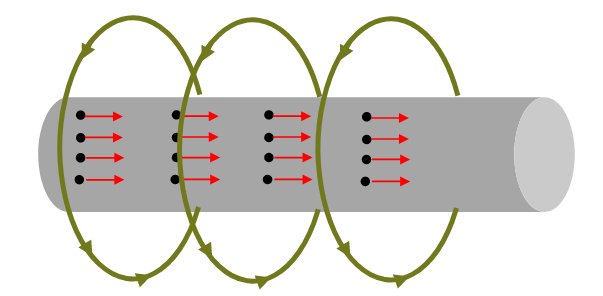
\includegraphics[scale=0.3]{img/hfeld.png}}

	\end{center}
	\definition{Magnetische Flussdichte \textbf{B}}
	\beginip
	Bewegte Ladungsträger welche sich in der Nähe anderer bewegter Ladungsträger befinden, verspüren eine Kraftwirkung welche senkrecht zur Bewegungsrichtung zeigt. \\
	Analog zum Elektrischen Feld definieren wir ein magnetisches Feld (= magnetische Flussdichte) welche diese Kraftwirkung beschreibt. \\
	Die Mangetische Flussdichte, weisst jedem Punkt im Raum einen Vektor zu. Die Resultierende Kraft auf ein Ladungsträger, welcher sich mit Geschwindigkeit V bewegt,
	berechnet sich aus dem Kreuzprodukt von Geschwindigkeit und Ladung ($\rightarrow$ \textbf{Lorentzkraft})
	\iend




	\definition{Rechte Hand Regel}
	\beginip
	Die magnetische Flussdichte $B$ um einen stromdurchflossenen Leiter baut sich stets gegen den Uhrzeigersinn auf und ist \textbf{immer geschlossen}. \\
	\begin{center}
			\ibox{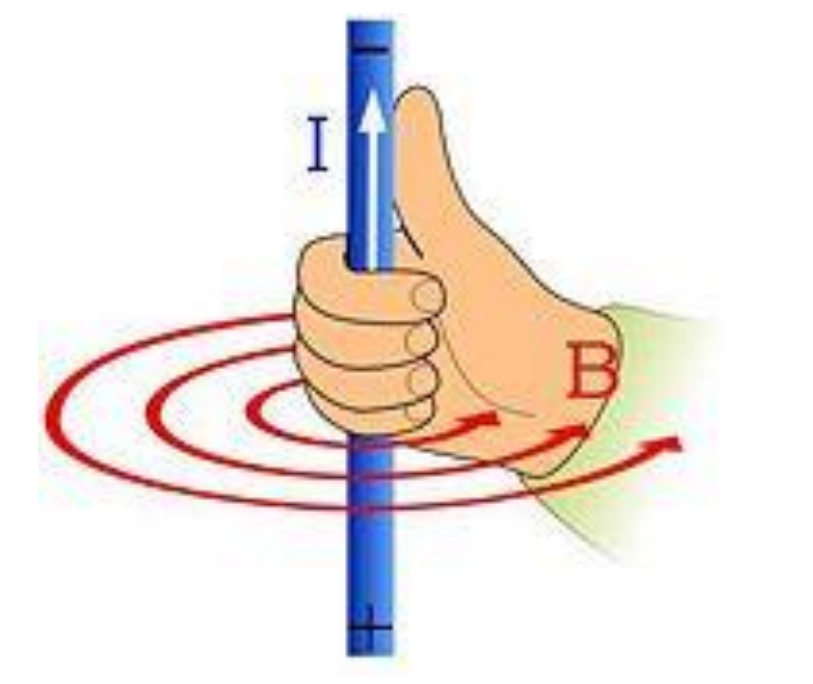
\includegraphics[scale=0.2]{img/rechte-hand-regel.png}}
	\end{center}
	\iend

 \newpage
	\gl{Gleichung}{Lorentzkraft}
	\begingl
	Bewegte Ladungen in einem Magnetfeld verspüren eine Kraft, welche proportional zur Stärke des B-Feldes und der Geschwindigkeit ist. \\
	Die Kraft steht senkrecht zu den Feld- und Geschwindigkeits-Vektoren.


	\begin{center}
			\ibox{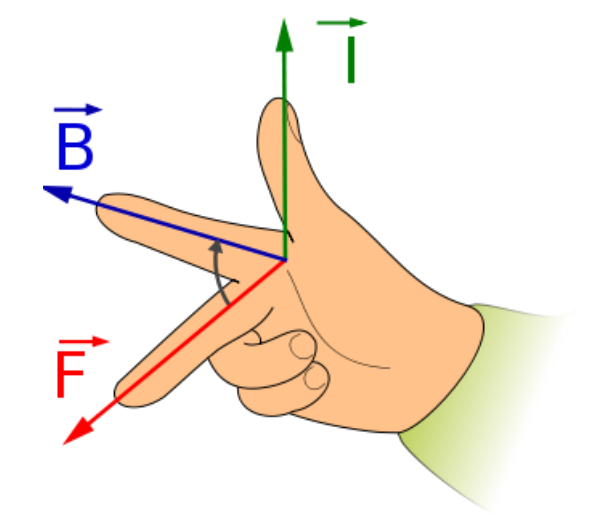
\includegraphics[scale=0.3]{img/lorentzkraft.png}}
	\end{center}

	\formulaBegin
	$\vec{F_m} = q \cdot \vec{v} \times \vec{B} = I(\vec{l} \times \vec{B})$
	\formulaEnd

	\textbf{Variabeln}: \\
	$ F_m = $ Magnetische Kraft $ [F_M] = N$ \\
	$ \vec{v} = $ Geschwindigkeit der Teilchen $ [v] = \frac{m}{s}$ \\
	$ \vec{B} = $ Magnetische Flussdichte $ [B] = T (Tesla)$ \\
	$ \vec{l} = $ Länge des Leiters im Magnetfeld $ [l] = m $\\

	Die Summe mit der Coulomb Kraft bezeichnet die \textbf{Lorentzkraft} \\

		\formulaBegin
		$\vec{F_L} = \vec{F_m} + \vec{F_c} = q \cdot \vec{v} \times \vec{B} = I(\vec{l} \times \vec{B}) + q \cdot \vec{E} $
		\formulaEnd

		In älteren Physikbüchern wird häufig nur die magnetische Kraftwirkung als Lorentzkraft bezeichnet.

	\iend

\newpage
	\definition{H-Feld}
	\beginip
	Legen wir ein magnetisches Feld an eine Materie an, so richten sich die eingeschlossenen Teile entgegen dem angelegten Feld aus und \texttt{"}schwächen\texttt{"} dieses. \\
	Das \texttt{"}abgeschwächte\texttt{"} Feld bezeichnen wir als magnetische Feldstärke (H-Feld) und entspricht dem Feld, welches real auf Ladungen wirkt. \\
	 Der \texttt{"}Abschwächungsfaktor\texttt{"} $\mu = \mu_0 \cdot \mu_r$ wird als Permeabilität bezeichnet. \\

	\formulaBegin
	$\displaystyle \vec{H} = \frac{\vec{B}}{\mu}$
	\formulaEnd

	\begin{center}
			\ibox{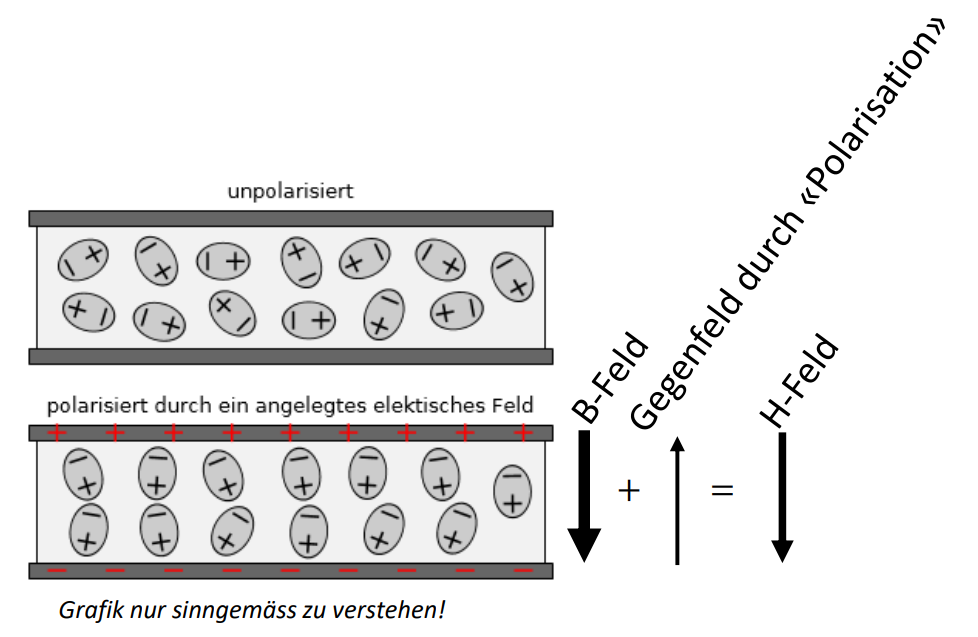
\includegraphics[scale=0.4]{img/h-feld.png}}
	\end{center}
	\iend

	\gl{Gleichung}{Durchflutungssatz}
	\begingl
	Der Durchflutungssatz sagt etwas darüber aus, wie das magnetische Feld entsteht. \\
	 Es bringt die \textbf{Magnetische Feldstärke H} (Feld) und den \textbf{Strom I} (Quelle) in Verbindung.
	Die Aussage des Durchflutungssatz ist, dass das Wegintegral des H-Feldes über eine beliebige \textbf{geschlossene} Kurve gerade dem Wert des durch diese Fläche fließenden Stromes entspricht. \\
	Diesen Wert definieren wir als Durchflutung $\Theta$ \\
	\formulaBegin
	$\displaystyle \Theta = \oint_{s} \vec{H} \cdot d\vec{s} = \iint_{A} \vec{j} \cdot d\vec{A} = I_{eff}$
	\formulaEnd
	Dabei ist es wichtig, das nur der \textbf{effektiv durch eine Fläche hindurchfliessende Strom} die Magnetische Durchflutung auslöst. Fliesst in einer Fläche gleich viel Strom hinein wie hinaus, ist die Durchflutung gleich 0.
	\iend

	\gl{Gleichung}{Vereinfachter Durchflutungssatz}
	\begingl
	Für den Fall, dass der Strom N mal durch eine Fläche hindurchfliesst und das H-Feld auf dem gesamten Weg konstant und parallel zum Weg ist, gilt folgende Vereinfachung:
	\formulaBegin
	$\displaystyle \Theta = H \cdot l_s = N\cdot I \rightarrow H = \frac{N \cdot I}{l_s}$
	\formulaEnd
	\iend

	\bsptask{Beispiel}{}
	\beginbsp
	Berechnen Sie die Durchflutung $\Theta$ und das H-Feld $\vec{H}$ um einen unendlich langen, mit Strom I durchflossenen Leiter. Der Radius des Leiters sei $\rho$. \\
	\iend
	\bsp{Lösung}{}
	\beginbsp
	Wir wählen als geschlossenen Weg einen Kreis mit Radius R um unseren Leiter. \\
	Da wir von einem perfekten Leiter ausgehen, treffen wir die Annahme, dass das Magnetfeld achsensymmetrisch und somit konstant entlang des Kreises ist. \\
	\\
	Wir erhalten: für R $ > \rho$: \\
	$\displaystyle  \doubleunderline{\Theta} =  \oint_{2\pi R} \vec{H} \cdot d\vec{S} = \doubleunderline{I} $ \\
	$ \displaystyle \rightarrow |H| \cdot 2 \pi R = I \rightarrow \doubleunderline{\vec{H}(R) = \frac{I}{2 \pi R} \cdot \vec{e_{\varphi}}} $\\

	Für R $ < \rho $ : \\
	$\displaystyle  \doubleunderline{\Theta(R)} =  \oint_{2\pi R} \vec{H} \cdot d\vec{S} =\int_{0}^{R} \int_{0}^{2\pi} \frac{I}{\pi{\rho}^2} \cdot r \cdot d\varphi  \cdot dr  = \frac{2 \cdot I}{\rho^2} \cdot \frac{1}{2} R^2 =  \doubleunderline{\frac{R^2\cdot I}{\rho^2}} 		  $ \\
	$ \displaystyle \rightarrow |H| \cdot 2 \pi R = \frac{I \cdot R^2}{\rho^2} \rightarrow \doubleunderline{\vec{H}(R) = \frac{I}{2\pi \rho^2} \cdot R \cdot \vec{e_{\varphi}}} $

	\textbf{Skizze}
	\begin{center}
		\ibox{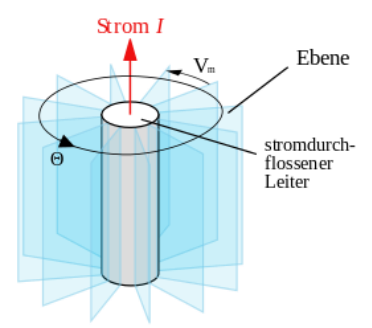
\includegraphics[scale=0.7]{img/ex4-1.png}}
	\end{center}
	\iend

	\bsptask{Beispiel}{Magnetfeld einer Spule}
	\beginbsp
	Gegeben sei eine Spule mit N Wicklungen und der länge l. Berechnen Sie die magnetische Feldstärke $\vec{H}$ in Abhängigkeit des Stromes I, Länge l und Wicklungen N.
\begin{center}

		\ibox{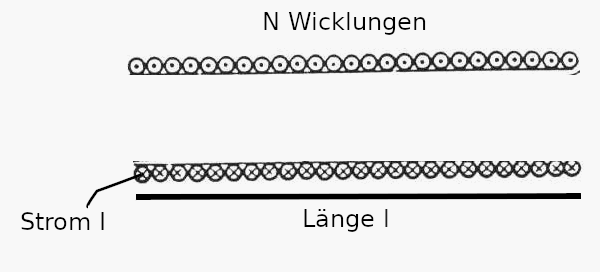
\includegraphics[scale=1.3]{img/ex-spule}}
\end{center}





	\iend

	\beginbsp
	Es gilt für die Durchflutung bezüglich des roten Weges:

		\begin{center}
			\ibox{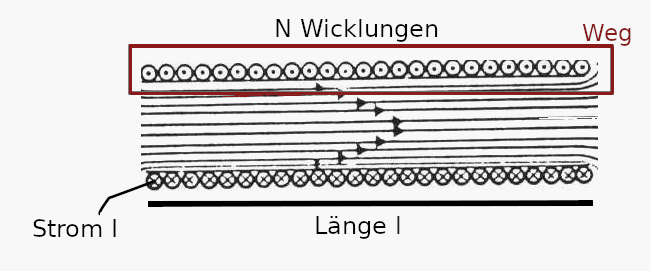
\includegraphics[scale=1.3]{img/spule-sol.png}}
		\end{center}





\begin{center}

	$\displaystyle \Theta_{Spule} = \oint_{s} \vec{H} \cdot d\vec{s} = \iint_{A_s} \vec{j} \cdot d\vec{A} = N \cdot I \simeq \int_0^b \vec{H} \cdot d\vec{s}$

	\end{center}
	Da die Anordnung \textbf{Symmetrisch zur X-Achse} ist, wird das H-Feld auf dem gesamten Weg konstant sein und in X-Richtung zeigen,
	\begin{center}

	$ \displaystyle \Theta_{Spule} = N \cdot I = H \cdot l_{s}$

	\end{center}
	Und somit gilt für das H-Feld mit Richtungsvektor:
	\begin{center}

	$\displaystyle H = \frac{N\cdot I}{l_{s}}  = \frac{N\cdot I}{l}$ \\ \fspace
 	$\displaystyle
		\doubleunderline{   \vec{H}(\vec{r}) =
		\begin{cases}
0 & $Aussherhalb der Spule $\\
\displaystyle \frac{N\cdot I}{l_{s}} \vec{e}_x & $Innerhalb der Spule $\\
\end{cases}}$

	\end{center}
	\iend


	Aus der letzten Aufgabe folgt, dass das magnetische Feld einer Spule im inneren Näherungsweise konstant ist. Ausserhalb der Windungen ist die Spule feldfrei. \\
	Diese Eigenschaften entsprechen gerade denen, eines \textbf{Stabmagneten}


\subsubsection{Verhalten von B und H Feld an Randflächen}
\fix \fix
\textbf{B-Feld} \\
Fliesst ein B-Feld durch einen Materialübergang, so verändert sich die \textbf{Tangentialkomponente}. Die \textbf{Normalkomponente} bleibt gleich.
\begin{center}
	\ibox{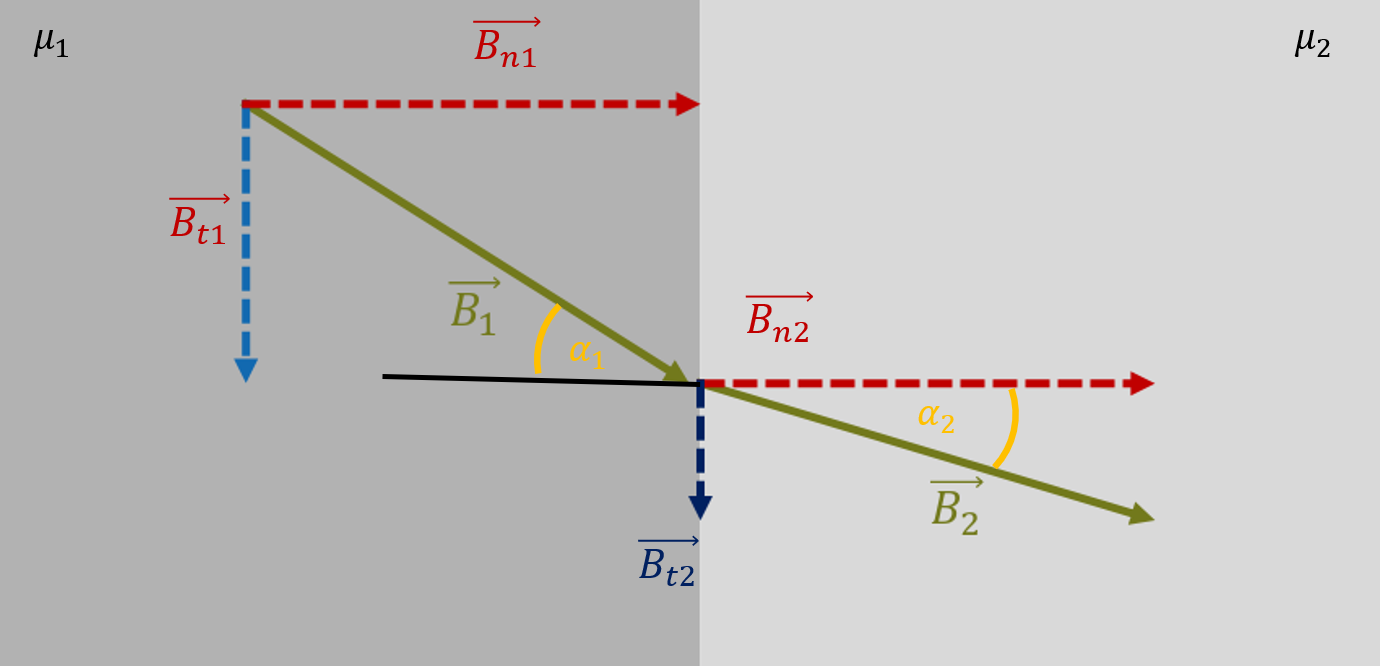
\includegraphics[scale=0.3]{img/brand}}
\end{center}

\formulaBegin
$ \displaystyle B_{n1} = B_{n2}$
\\ \fspace

 $\displaystyle B_{t2} = B_{t1} \frac{\mu_2}{\mu_1}  = \frac{tan(\alpha_2)}{tan(\alpha_1)}$
\formulaEnd

\textbf{H-Feld} \\
Fliesst ein H-Feld durch einen Materialübergang, so verändert sich die \textbf{Normalkomponente}. Die \textbf{Tangentialkomponente} bleibt gleich.

\begin{center}
	\ibox{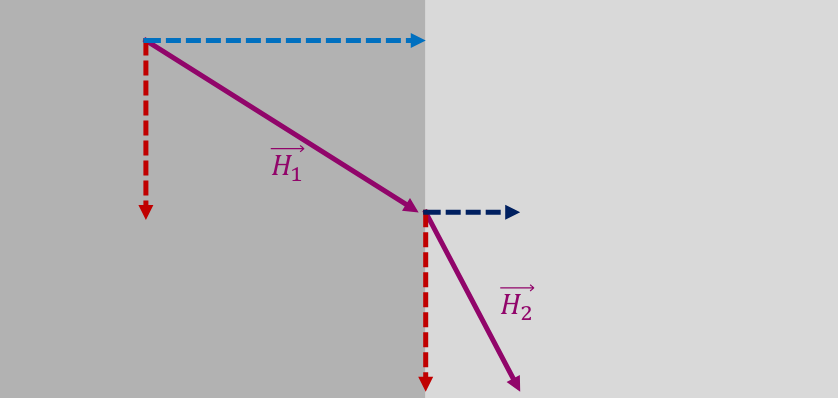
\includegraphics[scale=0.3]{img/hrand}}
\end{center}

\formulaBegin

$\displaystyle H_{n2} = H_{n1} \frac{\mu_1}{\mu_2} = \frac{tan(\alpha_1)}{tan(\alpha_2)} $ \\
\fspace
$ \displaystyle H_{t1} = H_{t2}$
\formulaEnd




\subsubsection{Das Reluktanzmodell}

	\definition{Magnetische Spannung}
	\beginip
	Als magnetische Spannung bezeichnen wir das Wegintegral über die magnetische Feldstärke H.
	\formulaBegin
	$\displaystyle V_{M_{AB}} := \int_A^B \vec{H} \cdot d\vec{s}$
	\formulaEnd

	Die magnetische Spannung ist einzig eine Hilfsgrösse, um Werte zu berechnen. \\
	Analog zum elektrischen Feld, lässt sich auch hier eine Maschengleichung definieren: \\
	\begin{center}
		$\displaystyle \oint_{Masche} \vec{H} \cdot d\vec{s} = \Theta_{Masche}$
	\end{center}
		Falls wir nun die Durchflutung $\Theta$ als Quelle einfügen, gilt für ein magnetisches Netzwerk:
		\begin{center}
			$\displaystyle \oint_{Masche} \vec{H} \cdot d\vec{s} + \Theta_{Quellen} = 0$
		\end{center}
	\iend

	\definition{Magnetischer Fluss}
	\beginip
		Als magnetischen Fluss $\Phi$ bezeichnen wir die \texttt{"}Menge B-Feld\texttt{"}, welche durch eine gegebene Fläche fliesst. \\
		\formulaBegin
		$\displaystyle \Phi := \iint_A \vec{B}  \cdot d\vec{A} \simeq \pm B \cdot A, \ \ \ [\Phi] = T	\cdot m^2 $
		\formulaEnd
	\iend





	\definition{Magnetischer Widerstand}
		\beginip
			Als magnetischer Widerstand $R_m$ bezeichnen wir das Verhältnis zwischen magnetischer Spannung und magnetischem Fluss \\
			Er sagt etwas darüber aus, wie gross der magnetische Fluss bei einer gegebenen magnetischen Spannung ist.
			\formulaBegin
			$\displaystyle R_m = \frac{V_M}{\Phi} \underbrace{=}_{magn. Leiter} \frac{l}{\mu \cdot A}$
			\formulaEnd
		\iend

		\textbf{Begründung} \\
		Wir gehen davon aus, dass die magnetische Spannung über einem Leiter mit Länge l anliegt, dessen Querschnittfläche A ist. \\
		\begin{center}
			$\displaystyle \frac{V_M}{\Phi} = \frac{\int_0^l \vec{H} \cdot d\vec{s}}{\iint_a \vec{B} d \vec{A}} = \frac{l \cdot H}{\mu \cdot A \cdot H} = \frac{l}{\mu \cdot A} $

		\end{center}


\newpage

		\textbf{magnetische Grössen im Vergleich zu eletrischen} \\

		\def\arraystretch{2}%  1 is the default, change whatever you need
		\begin{tabular}{c|c|c||c|c}
			& Elektrisch & Einheit & Magnetisch & Einheit \\
			\hline
			\hline
			Leitfähigkeit & $ \kappa $ & $\texttt{[}   \frac{1}{\Omega \cdot m}    \texttt{]}$ & $\mu (= \mu_0 \cdot \mu_r)$ & $\texttt{[}  \frac{H}{m}\texttt{]}$ \\
			Widerstand & $ R = \frac{l}{\kappa A} $ & $\texttt{[}   \Omega   \texttt{]}$ & $R_m = \frac{l}{\mu A}$ & $\texttt{[} \frac{1}{H}\texttt{]}$ \\
			Leitwert & $ G = \frac{1}{R} $ & $\texttt{[}  S \texttt{]}$ & $\Lambda_m = \frac{1}{R_m}$ & $\texttt{[}  H  \texttt{]}$ \\
			\hline


			Spannung & $\displaystyle U_{AB} = \int_A^B \vec{E} \cdot d\vec{s}$ & $\texttt{[}V\texttt{]}$ & $\displaystyle \Theta_{AB}= \int_A^B \vec{H} \cdot d\vec{s}$ &  $\texttt{[}A\texttt{]}$ \\
			Strom / Fluss & $\displaystyle I = \iint_A \vec{j}\cdot d\vec{A} = \kappa \iint_A \vec{E} \cdot d\vec{A}$ & $\texttt{[}A\texttt{]}$  & $ \iint_A \vec{B} \cdot d \vec{A} = \mu \iint_A \vec{H} \cdot d\vec{A}$ &  $\texttt{[}Wb\texttt{]}$ \\
			\hline
			Ohmsches Gesetz & $U = R \cdot I $ &  & $\Theta = R_m \cdot \Phi $ &  \\
			Maschenregel & $ U_0 = \sum_{Masche} U_m $ &  & $ \Theta(= NI) = \sum_{Masche} V_m $ & \\
			Knotenregel & $ \sum_{Knoten} I_k = 0 $ &  & $ \sum_{Knoten} \Phi_k = 0 $ &  \\

		\end{tabular}

		\definition{Reluktanzmodell}
		\beginip
		Das Reluktanzmodel besagt, dass man eine magnetische Anordnung, als elektrisches Schaltbild beschreiben und berechnen kann.
		\textbf{Vorgehen} \\
		\begin{itemize}
			\item Spulen werden mit Spannungsquellen ersetzt $V_m = N\cdot I$
			\item Magnetkerne/Luftspälte etc. werden mithilfe der Länge und Querschnittsfläche als Widerstände modelliert. $R_m =  \frac{l}{\mu \cdot A}$
			\item Für magnetische Widerstände gelten die gleichen Regeln wie bei elektrischen (Seriellschaltung / Paralellschaltung).
		\end{itemize}

		\iend
\newpage
		\bsptask{Beispiel}{}
		\beginbsp
 		\textbf{Aufgabe Hubmagnet} \\
		Der mittlere Schenkel (2) eines E-Kernes aus Dynamoblech trägt eine Wicklung mit N Windungen. Über
		die drei Luftspalten mit gleicher Länge $\delta$ wird ein Anker aus Grauguss mit der Kraft FA angezogen
		E-Kern und Anker besitzen die gleiche Dicke d. \\
		\begin{center}
		\ibox{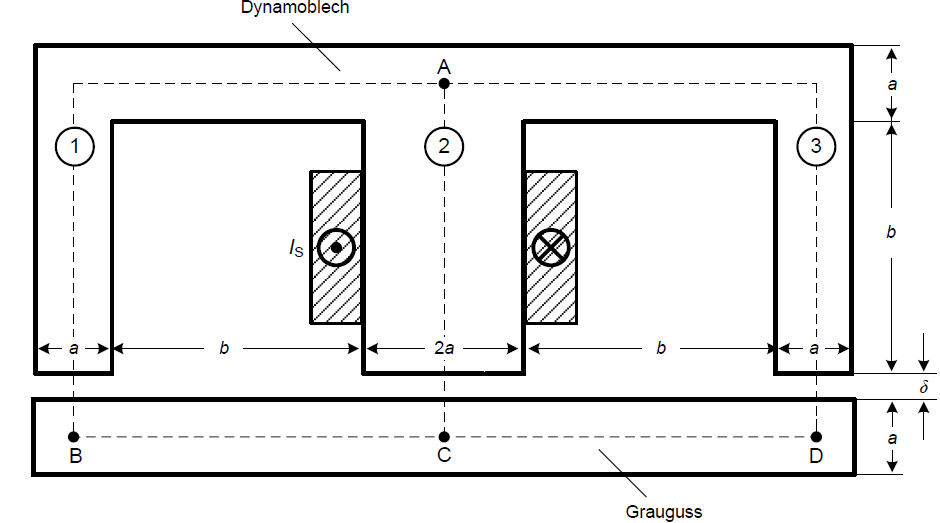
\includegraphics[scale=0.4]{img/ex5-1.png}}
		\end{center}
		Gegeben sind folgende Parameter: \\

		\begin{center}
	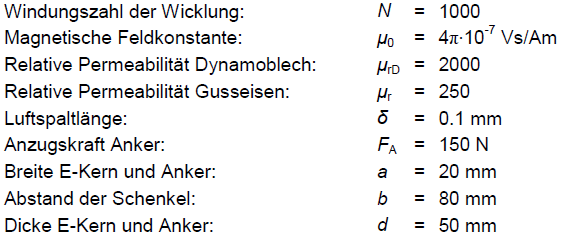
\includegraphics[scale=0.6]{img/ex5-3.png}
		\end{center}
		Berechnen sie die magnetische Spannung auf dem Weg ACD.
		\iend

\newpage
		\important{Lösung}{}
				\beginbsp
		Zuerst zeichnen wir ein Reluktanzmodell des Magneten. \\
		Wobei $R_L$ die Luftspälte, ${R_D}_i$ die Beine des Magneten und ${R_G}_i$ sowie $R_{BC}$ und $R_{CD}$ das Gusseinsenstück modellieren.


			\begin{minipage}[t]{0.55\textwidth}
						\ibox{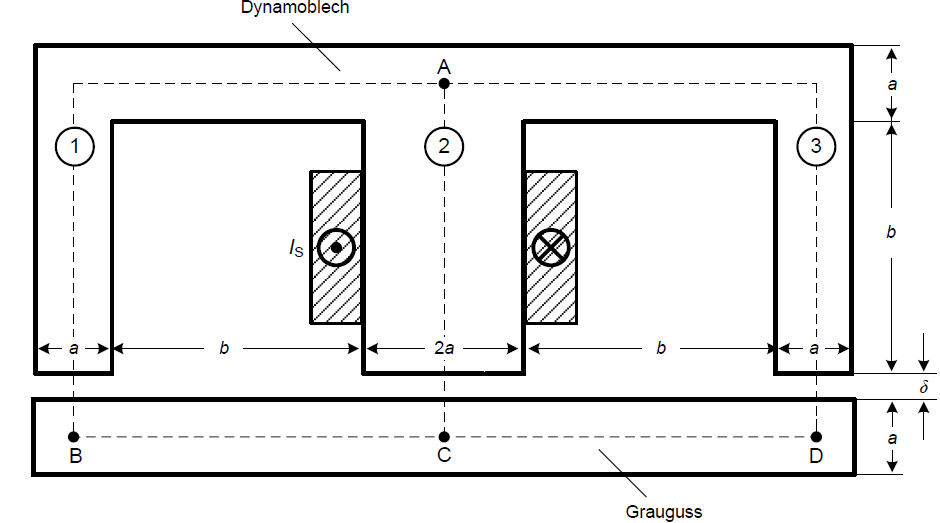
\includegraphics[scale=0.3]{img/ex5-1.png}}
\end{minipage}
			\begin{minipage}[t]{0.05\textwidth}
				\begin{center}
					\vspace{-3cm}
				$\Rightarrow$ \\

				\fspace
				\fspace
				\end{center}
			\end{minipage}
\begin{minipage}[t]{0.29\textwidth}
			\ibox{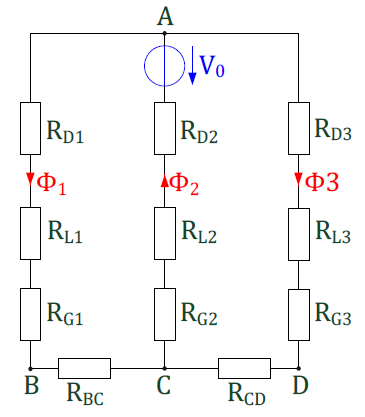
\includegraphics[scale=0.5]{img/ex5-2.png}}
\end{minipage}



		Für die Spannungsquelle erhalten wir:
			\begin{center}

				 $V_0 = N \cdot I_s = 1000 \cdot 211.3mA = 211.3A$ \\
			\end{center}
		Für die Widerstände:
			\begin{center}
	 	$R_{D1} = R_{D3} = \frac{2b + 2a}{\mu_0 \mu_{rD} a d} = 79.6 \cdot 10^3H^{-1}$ \\
	 	$R_{D2} = \frac{b + \frac{a}{2} }{2 \mu_0 \mu_{rD} a d} = 17.9 \cdot 10^3H^{-1}$ \\

	 	$R_{L1} = R_{L3} = \frac{\delta}{\mu_0 a d} = 79.6 \cdot 10^3H^{-1}$ \\
		$R_{L2} =  \frac{\delta}{2\mu_0 a d} = 39.8 \cdot 10^3 H^{-1}$\\
		$R_{G1} = R_{G3} = \frac{\frac{a}{2}}{\mu_0\mu_{rG}ad} = 31.8 \cdot 10^3H^{-1}$ \\
		$R_{G2} =\frac{\frac{a}{2}}{2\mu_0\mu_{rG}ad} = 15.9 \cdot 10^3H^{-1}$ \\
		$R_{BC} = R_{CD} = \frac{b + \frac{3}{2}a}{2\mu_0\mu_{rG}ad} = 350.1\cdot 10^3H^{-1}$ \\
				\end{center}
		Weiter können wir die einzelnen Widerstände seriell zusammenfassen:
			\begin{center}
		$R_1 = R_{D1} + R_{L1} + R_{G1} = 191 \cdot 10^3 H^{-1}$ \\
		$R_2 = R_{D2} + R_{L2} + R_{G2} = 73.7 \cdot 10^3 H^{-1}$ \\
		$R_3 = R_{D3} + R_{L3} + R_{G3} = 191 \cdot 10^3 H^{-1}$ \\
		$R_E = R_{BC} = R_ {CD} = 350.1 \cdot 10^3 H^{-1} $ \\
					\end{center}

		Die Spannung $U_{AC}$ lässt sich als Spannungsteiler berechnen:

			\begin{center}
		$\displaystyle U_{AC} = U_0 \cdot \frac{((R_1 + R_E) || (R_3 + R_E)) } { ((R_1 + R_E) || (R_3 + R_E)) + R_2} = 166A$ \\
				\end{center}
		Und somit die Spannung $ U_{AD}$:
		\begin{center}
			$\displaystyle \doubleunderline{U_{AD}} = 166A \cdot \frac{R_1}{R_1 + R_E} = \doubleunderline{58.6A}$
		\end{center}
		\iend

\newpage

\subsection{Spule und Induktivität}

\definition{Induktivität}
\beginip
	Die Induktivität L beschreibt, wieviel magnetischer Fluss $\Phi$ sich bei einem Strom I im Inneren eines Bauteiles aufbaut.
	\formulaBegin
	$ \displaystyle L := \frac{N\cdot \Phi}{I} = \frac{N^2}{R_m} $
	\formulaEnd
	Der Faktor $N$ im Nenner kommt daher, dass der Fluss bei einer Spule durch $N$ Windungen hindurchfliesst. Somit ist die effektive Fläche des Flusses N mal grösser, wesshalb er N mal gezählt wird. \\

	Die in einer Induktivität gespeicherte Energie berechnet sich zu
	\formulaBegin
	$W =\displaystyle \frac{1}{2}L \cdot I^2$
	\formulaEnd
\iend



\bsptask{Beispiel}{Berechnen einer Induktivität}
\beginbsp
Auf einem Ringkern mit der Querschnittsfläche A und der Permeabilität $\mu_r \rightarrow \infty$ ist
eine Wicklungen mit $N_1$ Windungen angebracht. Der Ringkern
besitzt einen Luftspalt mit der sehr kleinen Breite $l_g$. Das magnetische Feld kann im
Luftspalt als homogen angenommen werden.

1) Berechnen sie die magnetische Flussdichte im Luftspalt. \\
2) Berechnen sie den magnetischen Fluss $\phi_A$ im Kern.\\
3) Berechnen sie die Induktivität L
\begin{center}

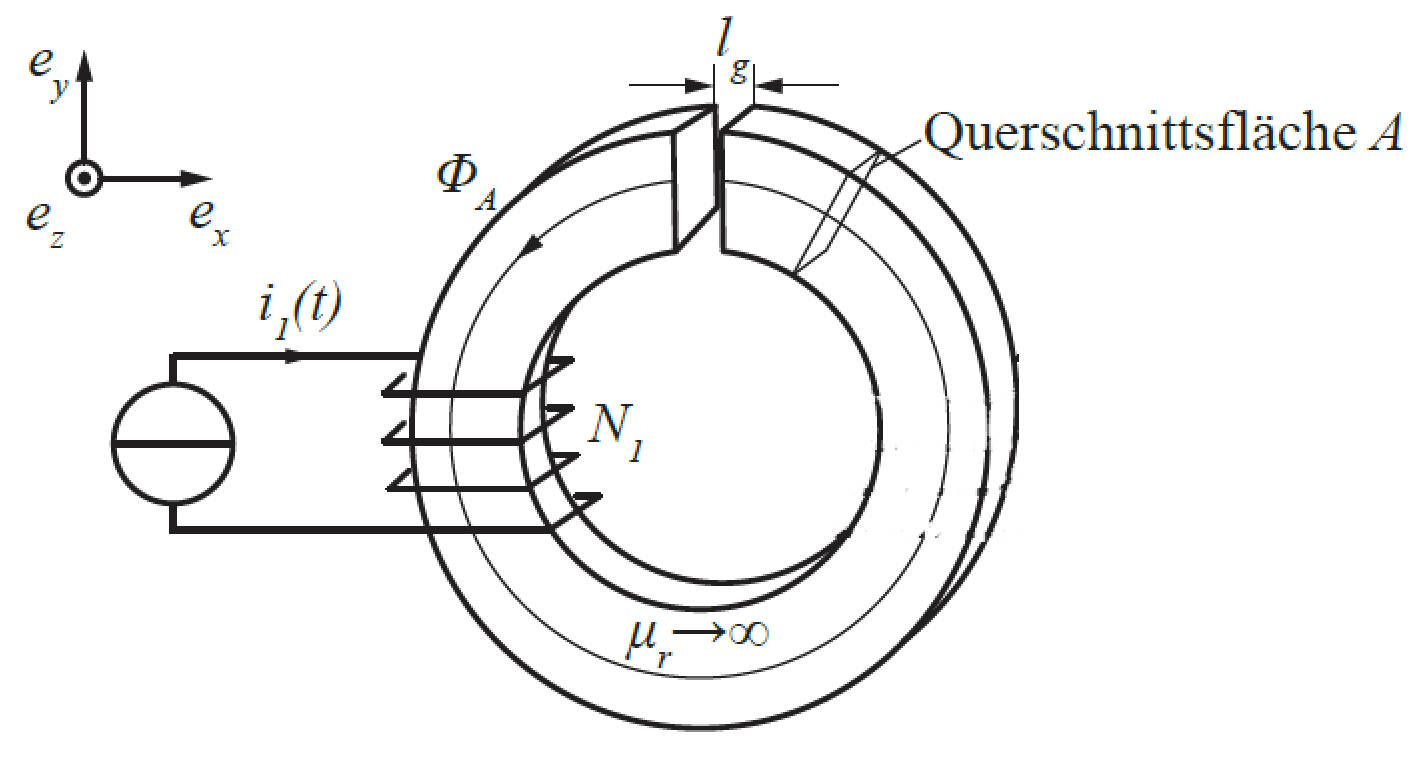
\includegraphics[scale=0.25]{img/induktivitaet_bsp_1.PNG}

\end{center}

\iend
\newpage

\bsp{Lösung}{}

\beginbsp
\begin{itemize}
\item 1) Es gilt für die Durchflutung bezüglich dem Kreisring:
			\begin{center}
				$\Theta =  \oint_s \vec{H}\cdot d\vec{s} = N_1\cdot i_1(t)$
			\end{center}
			Da die Permeabilität des Magneten gegen unendlich strebt und das B-Feld bei senkrechten Materialübergängen konstant ist gilt: \\

			\begin{center}
			$\displaystyle \oint_s \vec{H} d\vec{s} = \underbrace{\int_{M} \frac{\vec{B}}{\mu_0 \cdot \mu_r} d\vec{s}}_{=0} + \int_{L} \frac{\vec{B}}{\mu_0} d\vec{s} = \int_{L} \frac{\vec{B}}{\mu_0} d\vec{s} $
		\end{center}
		Da des B-feld parallel zum Weg ist und über dem ganzen Weg konstant ist gilt:
		\begin{center}
				$\displaystyle N_1 \cdot i_1(t) = \displaystyle \oint_s \vec{H} d\vec{s} = \frac{B}{\mu_0} \cdot l_g$ \\
				$\displaystyle \rightarrow \doubleunderline{\vec{B} = \frac{N_1 \cdot i_1(t) \mu_0}{l_g} (-\vec{e}_x)}$
		\end{center}

		\item 2) Für den magnetischen Fluss gilt:
		\begin{center}
				$\displaystyle \phi_A = \iint_A \vec{B} \cdot d\vec{A} = B \cdot A =\doubleunderline{\frac{N_1 \cdot i_1(t) \mu_0}{l_g} \cdot A}$
		\end{center}

		\item 3) Da die Spule $N_1$ Wicklungen aufweist, muss der Fluss $\phi_A$ genau $N_1$ mal gezählt werden. Es gilt für die Induktivität:
		\begin{center}
				$ \displaystyle L:= {\phi}{i} = N_1 \cdot  \frac{N_1 \cdot i_1(t) \mu_0}{l_g} \cdot A \cdot \frac{1}{i_1(t)} =  \doubleunderline{\frac{N_1^2 \cdot \mu_0}{l_g} \cdot A}$
		\end{center}
\end{itemize}

\iend




	\definition{Serien und Parallelschaltung}
	 \beginip
	 	Induktivitäten verhalten sich analog zu Widerständen: \\
		\textbf{Serienschaltung}
		\formulaBegin
		$ L_{serie} = \sum_{i=0}^n L_i $
		\formulaEnd

		\textbf{Parallelschaltung}
		\formulaBegin
		$\displaystyle \frac{1}{L_{par}} = \sum_{i=0}^n \frac{1}{L_i} \Bigg\rvert L_{par} = (L_1 || L_2 )$
		\formulaEnd
	 \iend
\newpage


\definition{Gegeninduktivität}
\beginip
Die Gegeninduktivität beschreibt, wie viel magnetischer Fluss durch eine \textbf{andere} Leiterschleife durchfliesst, abhängig
des Stromes in der ersten Schleife.
\formulaBegin
$\displaystyle L_{21} = N_2 \cdot \frac{\phi_{21}}{i_1}$
\formulaEnd
\begin{center}

	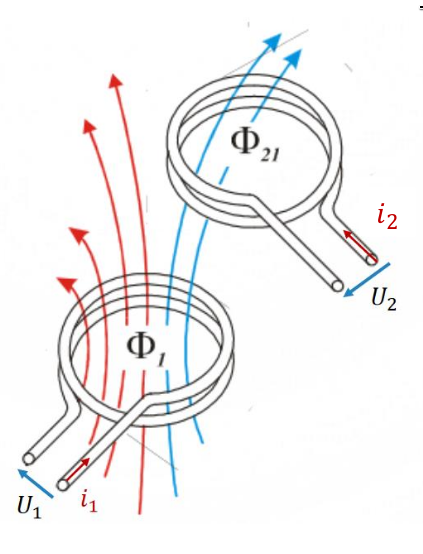
\includegraphics[scale=0.3]{img/gegenind}
\end{center}
\iend


\bsptask{Beispiel}{Berechnen einer Gegeninduktivität}
\beginbsp
Beim Ringkern aus dem vorherigen Beispiel wird nun eine 2 Spule mit $N_2$ Wicklungen hinzugefügt. Berechnen sie die Gegeninduktivität $L_{21}$ bezüglich der Spule mit den $N_2$ Windungen.
\begin{center}

	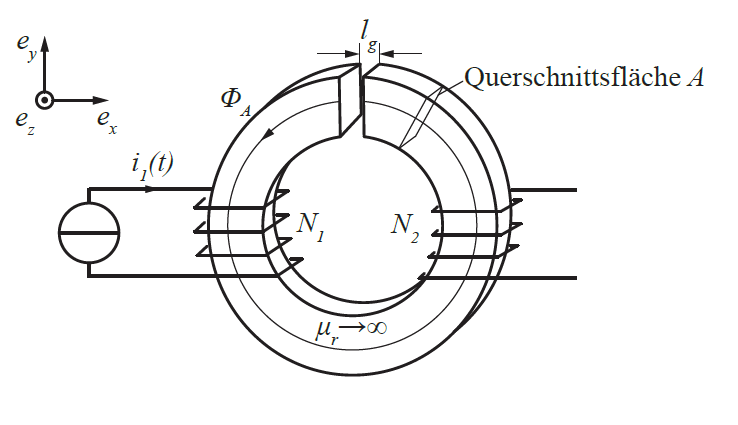
\includegraphics[scale=0.5]{img/induktivitaet_bsp_2.png}
\end{center}
\iend

\newpage


\bsp{Lösung}{}
\beginbsp

Die Gegeninduktivität beschreibt, wieviel magnetischer Fluss durch die 2. Spule fliesst abhängig des Stromes der ersten Spule:
\begin{center}
$\displaystyle L_{21} := \frac{\Phi_{21}}{i_1}$
\end{center}

Da der Fluss im Magneten selbst gerade $\Phi_A$ beträgt und dieser durch $N_2$ Leiterschleifen fliesst, gilt:
\begin{center}

	$\displaystyle  L_{21} := \frac{\Phi_{21}}{i_1} = \frac{\Phi_A \cdot N_2}{i_1} = \doubleunderline{\frac{N_1\cdot N_2 \cdot \mu_0}{l_g} \cdot A}$
\end{center}
\iend






%	\textbf{Übersicht} \\
%	\\
%	\begin{tabular}{|c|c|c|c|c|}
%	\hline
%		\textbf{Energie} & 	\textbf{Strom und Spannung} & 	\textbf{ DC-Verhalten} & 	\textbf{ High-AC Verhalten*}& 	\textbf{ Admitanz*} \\
%		\hline 	\hline
%		 & & & & \\
%	    $ \displaystyle L =  \frac{N \Phi}{I} $ & $\displaystyle i_L(t) = \frac{1}{L} \int_0^t u_c(t) dt $ & Leerlauf & Kurzschluss & $ \displaystyle j\omega L$  \\
%		  $\displaystyle W =  \frac{1}{2} L I^2 $ & $\displaystyle u_L(t) = L \cdot \frac{d}{d t} (i_c) $ & 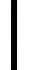
\includegraphics[scale=0.5]{img/kurzschluss} &   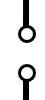
\includegraphics[scale=0.4]{img/leerlauf}  &   \\
%			 & & & & \\
%			\hline
%	\end{tabular}
